%----------------------------------------------------------------------------------------
%	PACKAGES AND OTHER DOCUMENT CONFIGURATIONS
%----------------------------------------------------------------------------------------

\documentclass{article}

\usepackage{fancyhdr} % Required for custom headers
\usepackage{lastpage} % Required to determine the last page for the footer
\usepackage{extramarks} % Required for headers and footers
\usepackage{graphicx} % Required to insert images
\usepackage{listings}
\usepackage{color}
\usepackage{xcolor}
\usepackage{caption}
\usepackage{enumitem}
\usepackage{amsmath}
\usepackage{tikz}
\usetikzlibrary{calc,shapes.multipart,chains,arrows}

\DeclareCaptionFont{white}{\color{white}}
\DeclareCaptionFormat{listing}{%
\parbox{\textwidth}{\colorbox{gray}{\parbox{\textwidth}{#1#2#3}}\vskip-4pt}}
\captionsetup[lstlisting]{format=listing,labelfont=white,textfont=white}

% Margins
\topmargin=-0.45in
\evensidemargin=0in
\oddsidemargin=0in
\textwidth=6.5in
\textheight=9.0in
\headsep=0.25in 

\linespread{1.1} % Line spacing

% Set up the header and footer
\pagestyle{fancy}
\lhead{\hmwkAuthorName} % Top left header
\chead{\hmwkClass\ (\hmwkClassInstructor\ \hmwkClassTime): \hmwkTitle} % Top center header
\rhead{\hmwkDueDate} % Top right header
\lfoot{\lastxmark} % Bottom left footer
\cfoot{} % Bottom center footer
\rfoot{Page\ \thepage\ of\ \pageref{LastPage}} % Bottom right footer
\renewcommand\headrulewidth{0.4pt} % Size of the header rule
\renewcommand\footrulewidth{0.4pt} % Size of the footer rule

\setlength\parindent{0pt} % Removes all indentation from paragraphs

%----------------------------------------------------------------------------------------
%	DOCUMENT STRUCTURE COMMANDS
%	Skip this unless you know what you're doing
%----------------------------------------------------------------------------------------

\setcounter{secnumdepth}{0} % Removes default section numbers
\newcounter{homeworkProblemCounter} % Creates a counter to keep track of the number of problems

\newcommand{\homeworkProblemName}{}
\newenvironment{homeworkProblem}[1][Problem \arabic{homeworkProblemCounter}]{ % Makes a new environment called homeworkProblem which takes 1 argument (custom name) but the default is "Problem #"
\stepcounter{homeworkProblemCounter} % Increase counter for number of problems
\renewcommand{\homeworkProblemName}{#1} % Assign \homeworkProblemName the name of the problem
\section{\homeworkProblemName} % Make a section in the document with the custom problem count
}

%----------------------------------------------------------------------------------------
%   COLORS AND LANGUAGAGE
%----------------------------------------------------------------------------------------

\lstset{
    frame=lrb,xleftmargin=\fboxsep,xrightmargin=-\fboxsep,language=Java,basicstyle=\ttfamily,
    breaklines=true,columns=fullflexible,keepspaces=true,escapeinside={\%*}{*)}
       }

%----------------------------------------------------------------------------------------
%	NAME AND CLASS SECTION
%----------------------------------------------------------------------------------------

\newcommand{\hmwkTitle}{Homework\ \#1} % Assignment title
\newcommand{\hmwkDueDate}{ Thursday,\ September\ 10,\ 2015} % Due date
\newcommand{\hmwkClass}{COT\ 5310} % Course/class
\newcommand{\hmwkClassTime}{6:15pm} % Class/lecture time
\newcommand{\hmwkClassInstructor}{Bobadilla} % Teacher/lecturer
\newcommand{\hmwkAuthorName}{Musa V. Ahmed} % Your name

%----------------------------------------------------------------------------------------

\begin{document}
\belowcaptionskip=-10pt

%----------------------------------------------------------------------------------------
%	PROBLEM 1
%----------------------------------------------------------------------------------------

\begin{homeworkProblem}
    Solve Sipser exercises 0.3, 0.4, 0.5, and problem 0.10.

    \vspace{5 mm}
    0.3 
    \begin{enumerate}[label=\alph*.]
        \item No.
        \item Yes.
        \item ${x, y, z}$
        \item ${x, y}$
        \item ${xx, xy, yx, yy, zx, zy, xz, yz}$
        \item ${{x,y}, {x}, {y}}$
    \end{enumerate}

    0.4 The cartesian product has $a*b$ elements. Since the cartesian product is $b$ ordered 
    pairs for each of the $m$ elements.

    0.5 There are $2^c$ elements in the power set of $C$. Since the subsets in the power set 
    either include an element of $C$ or they do not then it holds that there are $2^|C|$ 
    elements in the power set.

    0.10 In the step where we divide both sides by $(a-b)$ if $a=b$ then $(a-b)=0$. This leads 
    to a divide by zero error.
\end{homeworkProblem}
\clearpage

%----------------------------------------------------------------------------------------

%----------------------------------------------------------------------------------------
%	PROBLEM 2
%----------------------------------------------------------------------------------------

\begin{homeworkProblem}
    For a DFA, $M=(Q,\sum, \delta, q_0, F)$ in which the set of states is $Q=\{q_1, q_2, q_3, q_4, q_5\}$, 
    $\sum = \{a, b\}$, $q_0=q_1$, $F=\{q_2, q_3, q_4, q_5\}$, and $\delta$ is specified by the table: \\

    \begin{center}
        \begin{tabular}{l | l | l | l | l | l}
            \hline
            $\delta$ & $q_1$ & $q_2$ & $q_3$ & $q_4$ & $q_5$ \\ \hline
            a & $q_1$ & $q_3$ & $q_5$ & $q_2$ & $q_4$ \\ \hline
            b & $q_2$ & $q_4$ & $q_1$ & $q_3$ & $q_5$ \\ \hline
        \end{tabular}
    \end{center}

    Do the following:
    \begin{enumerate}[label=(\alph*)]
        \item Draw the state diagram of the DFA.
        \item For the strings below, give the corresponding computation of the automaton 
            and say whether it accepts or rejects them. The definition of computation 
            is given in page 40.
            \begin{enumerate}
                \item baab
                \item abbb
                \item bbba
            \end{enumerate}
        \item Give a succinct English description of the string accepted by $M$.
    \end{enumerate}

    \vspace{5 mm}
    \begin{enumerate}[label=\alph*.]
        \item 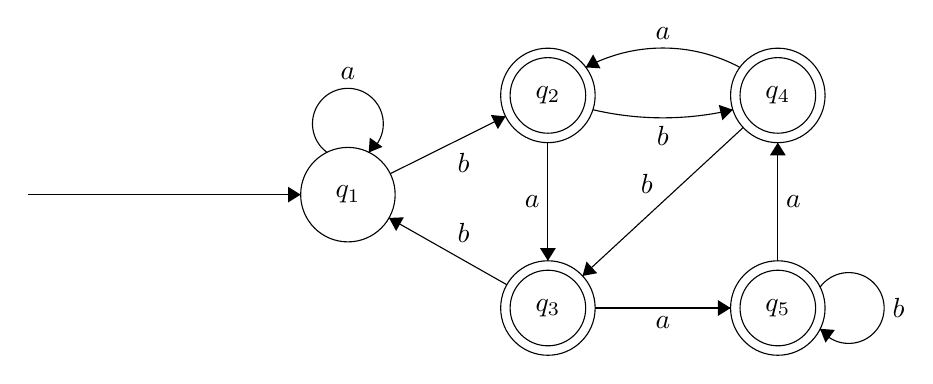
\begin{tikzpicture}[scale=0.2]
                    \tikzstyle{every node}+=[inner sep=0pt]
                    \draw [black] (20.3,-43.5) circle (3);
                    \draw (20.3,-43.5) node {$q_1$};
                    \draw [black] (33,-37.2) circle (3);
                    \draw (33,-37.2) node {$q_2$};
                    \draw [black] (33,-37.2) circle (2.4);
                    \draw [black] (33,-50.7) circle (3);
                    \draw (33,-50.7) node {$q_3$};
                    \draw [black] (33,-50.7) circle (2.4);
                    \draw [black] (47.6,-37.2) circle (3);
                    \draw (47.6,-37.2) node {$q_4$};
                    \draw [black] (47.6,-37.2) circle (2.4);
                    \draw [black] (47.6,-50.7) circle (3);
                    \draw (47.6,-50.7) node {$q_5$};
                    \draw [black] (47.6,-50.7) circle (2.4);
                    \draw [black] (0,-43.5) -- (17.3,-43.5);
                    \fill [black] (17.3,-43.5) -- (16.5,-43) -- (16.5,-44);
                    \draw [black] (18.977,-40.82) arc (234:-54:2.25);
                    \draw (20.3,-36.25) node [above] {$a$};
                    \fill [black] (21.62,-40.82) -- (22.5,-40.47) -- (21.69,-39.88);
                    \draw [black] (22.99,-42.17) -- (30.31,-38.53);
                    \fill [black] (30.31,-38.53) -- (29.37,-38.44) -- (29.82,-39.34);
                    \draw (27.64,-40.85) node [below] {$b$};
                    \draw [black] (33,-40.2) -- (33,-47.7);
                    \fill [black] (33,-47.7) -- (33.5,-46.9) -- (32.5,-46.9);
                    \draw (32.5,-43.95) node [left] {$a$};
                    \draw [black] (36,-50.7) -- (44.6,-50.7);
                    \fill [black] (44.6,-50.7) -- (43.8,-50.2) -- (43.8,-51.2);
                    \draw (40.3,-51.2) node [below] {$a$};
                    \draw [black] (45.4,-39.24) -- (35.2,-48.66);
                    \fill [black] (35.2,-48.66) -- (36.13,-48.49) -- (35.45,-47.75);
                    \draw (39.28,-43.46) node [above] {$b$};
                    \draw [black] (50.28,-49.377) arc (144:-144:2.25);
                    \draw (54.85,-50.7) node [right] {$b$};
                    \fill [black] (50.28,-52.02) -- (50.63,-52.9) -- (51.22,-52.09);
                    \draw [black] (35.402,-35.421) arc (118.22868:61.77132:10.355);
                    \fill [black] (35.4,-35.42) -- (36.34,-35.48) -- (35.87,-34.6);
                    \draw (40.3,-33.69) node [above] {$a$};
                    \draw [black] (30.39,-49.22) -- (22.91,-44.98);
                    \fill [black] (22.91,-44.98) -- (23.36,-45.81) -- (23.85,-44.94);
                    \draw (27.65,-46.6) node [above] {$b$};
                    \draw [black] (44.744,-38.108) arc (-76.77996:-103.22004:19.432);
                    \fill [black] (44.74,-38.11) -- (43.85,-37.8) -- (44.08,-38.78);
                    \draw (40.3,-39.12) node [below] {$b$};
                    \draw [black] (47.6,-47.7) -- (47.6,-40.2);
                    \fill [black] (47.6,-40.2) -- (47.1,-41) -- (48.1,-41);
                    \draw (48.1,-43.95) node [right] {$a$};
                \end{tikzpicture}
        \item $baab$ is accepted. $abbb$ is accepted. $bbba$ is accepted.

        \item It accepted strings that do not have four consecutive $b$'s.
    \end{enumerate}
\end{homeworkProblem}
\clearpage

%----------------------------------------------------------------------------------------

%----------------------------------------------------------------------------------------
%	PROBLEM 3
%----------------------------------------------------------------------------------------

\begin{homeworkProblem}
    For each of the following languages give a state diagram of a DFA that recognize it. 
    The alphabet is $\sum=\{0, 1\}$

    \begin{enumerate}[label=(\alph*)]
        \item \{$w|w$ does not contain 000 or 11 as a substring\}
        \item \{$w|w$ contain at least two 0's and at least two 1's\}. The 0's and 1's do not 
            need to be consecutive.
    \end{enumerate}

    \vspace{5 mm}
    \begin{enumerate}[label=(\alph*)]
        \item  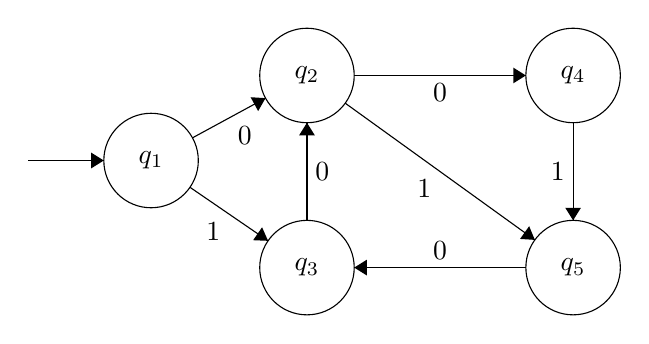
\begin{tikzpicture}[scale=0.2]
                \tikzstyle{every node}+=[inner sep=0pt]
                \draw [black] (30.2,-40.5) circle (3);
                \draw (30.2,-40.5) node {$q_1$};
                \draw [black] (40.1,-35.1) circle (3);
                \draw (40.1,-35.1) node {$q_2$};
                \draw [black] (40.1,-47.3) circle (3);
                \draw (40.1,-47.3) node {$q_3$};
                \draw [black] (57,-35.1) circle (3);
                \draw (57,-35.1) node {$q_4$};
                \draw [black] (57,-47.3) circle (3);
                \draw (57,-47.3) node {$q_5$};
                \draw [black] (22.4,-40.5) -- (27.2,-40.5);
                \fill [black] (27.2,-40.5) -- (26.4,-40) -- (26.4,-41);
                \draw [black] (32.83,-39.06) -- (37.47,-36.54);
                \fill [black] (37.47,-36.54) -- (36.52,-36.48) -- (37,-37.36);
                \draw (36.15,-38.3) node [below] {$0$};
                \draw [black] (43.1,-35.1) -- (54,-35.1);
                \fill [black] (54,-35.1) -- (53.2,-34.6) -- (53.2,-35.6);
                \draw (48.55,-35.6) node [below] {$0$};
                \draw [black] (42.53,-36.86) -- (54.57,-45.54);
                \fill [black] (54.57,-45.54) -- (54.21,-44.67) -- (53.63,-45.48);
                \draw (47.55,-41.7) node [below] {$1$};
                \draw [black] (57,-38.1) -- (57,-44.3);
                \fill [black] (57,-44.3) -- (57.5,-43.5) -- (56.5,-43.5);
                \draw (56.5,-41.2) node [left] {$1$};
                \draw [black] (54,-47.3) -- (43.1,-47.3);
                \fill [black] (43.1,-47.3) -- (43.9,-47.8) -- (43.9,-46.8);
                \draw (48.55,-46.8) node [above] {$0$};
                \draw [black] (40.1,-44.3) -- (40.1,-38.1);
                \fill [black] (40.1,-38.1) -- (39.6,-38.9) -- (40.6,-38.9);
                \draw (40.6,-41.2) node [right] {$0$};
                \draw [black] (32.67,-42.2) -- (37.63,-45.6);
                \fill [black] (37.63,-45.6) -- (37.25,-44.74) -- (36.68,-45.56);
                \draw (34.15,-44.4) node [below] {$1$};
            \end{tikzpicture}

        \item Draw Tikz here.
    \end{enumerate}
\end{homeworkProblem}
\clearpage

%----------------------------------------------------------------------------------------

%----------------------------------------------------------------------------------------
%	PROBLEM 4
%----------------------------------------------------------------------------------------

\begin{homeworkProblem}
    Solve Sipser exercises 1.6b, 1.6d, 1.5c, 1.4c.
    \begin{itemize}
        \item 1.6b \{$w|w$ begins with a 1 and ends with a 0\} \\
            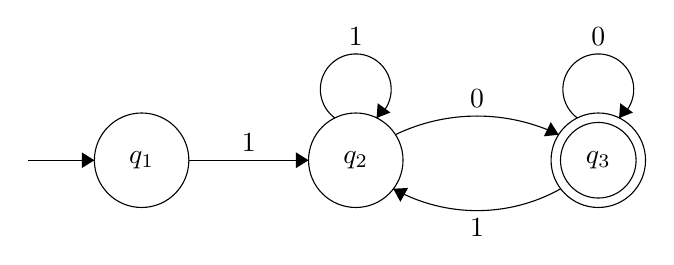
\begin{tikzpicture}[scale=0.2]
            \tikzstyle{every node}+=[inner sep=0pt]
            \draw [black] (26.6,-34.1) circle (3);
            \draw (26.6,-34.1) node {$q_1$};
            \draw [black] (40.2,-34.1) circle (3);
            \draw (40.2,-34.1) node {$q_2$};
            \draw [black] (55.6,-34.1) circle (3);
            \draw (55.6,-34.1) node {$q_3$};
            \draw [black] (55.6,-34.1) circle (2.4);
            \draw [black] (19.4,-34.1) -- (23.6,-34.1);
            \fill [black] (23.6,-34.1) -- (22.8,-33.6) -- (22.8,-34.6);
            \draw [black] (29.6,-34.1) -- (37.2,-34.1);
            \fill [black] (37.2,-34.1) -- (36.4,-33.6) -- (36.4,-34.6);
            \draw (33.4,-33.6) node [above] {$1$};
            \draw [black] (38.877,-31.42) arc (234:-54:2.25);
            \draw (40.2,-26.85) node [above] {$1$};
            \fill [black] (41.52,-31.42) -- (42.4,-31.07) -- (41.59,-30.48);
            \draw [black] (42.713,-32.476) arc (115.6864:64.3136:11.967);
            \fill [black] (53.09,-32.48) -- (52.58,-31.68) -- (52.15,-32.58);
            \draw (47.9,-30.79) node [above] {$0$};
            \draw [black] (53.219,-35.909) arc (-60.68763:-119.31237:10.864);
            \fill [black] (42.58,-35.91) -- (43.03,-36.74) -- (43.52,-35.86);
            \draw (47.9,-37.8) node [below] {$1$};
            \draw [black] (54.277,-31.42) arc (234:-54:2.25);
            \draw (55.6,-26.85) node [above] {$0$};
            \fill [black] (56.92,-31.42) -- (57.8,-31.07) -- (56.99,-30.48);
        \end{tikzpicture}

        \item 1.6d \{$w|w$ has length at least 3 and its third symbol is 0\} \\
            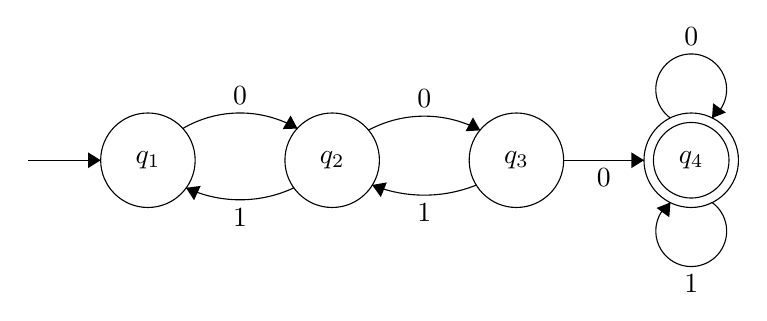
\begin{tikzpicture}[scale=0.2]
                \tikzstyle{every node}+=[inner sep=0pt]
                \draw [black] (21.1,-35.8) circle (3);
                \draw (21.1,-35.8) node {$q_1$};
                \draw [black] (32.8,-35.8) circle (3);
                \draw (32.8,-35.8) node {$q_2$};
                \draw [black] (44.5,-35.8) circle (3);
                \draw (44.5,-35.8) node {$q_3$};
                \draw [black] (55.6,-35.8) circle (3);
                \draw (55.6,-35.8) node {$q_4$};
                \draw [black] (55.6,-35.8) circle (2.4);
                \draw [black] (23.3,-33.792) arc (120.45553:59.54447:7.202);
                \fill [black] (30.6,-33.79) -- (30.16,-32.96) -- (29.66,-33.82);
                \draw (26.95,-32.3) node [above] {$0$};
                \draw [black] (30.382,-37.546) arc (-64.8218:-115.1782:8.067);
                \fill [black] (23.52,-37.55) -- (24.03,-38.34) -- (24.45,-37.43);
                \draw (26.95,-38.81) node [below] {$1$};
                \draw [black] (13.5,-35.8) -- (18.1,-35.8);
                \fill [black] (18.1,-35.8) -- (17.3,-35.3) -- (17.3,-36.3);
                \draw [black] (35.092,-33.896) arc (118.27212:61.72788:7.511);
                \fill [black] (42.21,-33.9) -- (41.74,-33.08) -- (41.27,-33.96);
                \draw (38.65,-32.5) node [above] {$0$};
                \draw [black] (41.962,-37.372) arc (-67.9611:-112.0389:8.826);
                \fill [black] (35.34,-37.37) -- (35.89,-38.14) -- (36.27,-37.21);
                \draw (38.65,-38.52) node [below] {$1$};
                \draw [black] (47.5,-35.8) -- (52.6,-35.8);
                \fill [black] (52.6,-35.8) -- (51.8,-35.3) -- (51.8,-36.3);
                \draw (50.05,-36.3) node [below] {$0$};
                \draw [black] (54.277,-33.12) arc (234:-54:2.25);
                \draw (55.6,-28.55) node [above] {$0$};
                \fill [black] (56.92,-33.12) -- (57.8,-32.77) -- (56.99,-32.18);
                \draw [black] (56.923,-38.48) arc (54:-234:2.25);
                \draw (55.6,-43.05) node [below] {$1$};
                \fill [black] (54.28,-38.48) -- (53.4,-38.83) -- (54.21,-39.42);
            \end{tikzpicture}

        \item 1.5c \{$w|w$ contains neither the substrings $ab$ nor $ba$\} \\
            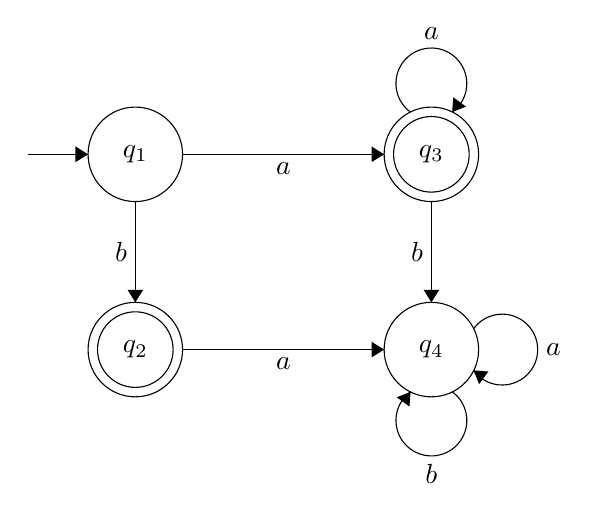
\begin{tikzpicture}[scale=0.2]
                \tikzstyle{every node}+=[inner sep=0pt]
                \draw [black] (25.5,-31) circle (3);
                \draw (25.5,-31) node {$q_1$};
                \draw [black] (44.3,-31) circle (3);
                \draw (44.3,-31) node {$q_3$};
                \draw [black] (44.3,-31) circle (2.4);
                \draw [black] (25.5,-43.4) circle (3);
                \draw (25.5,-43.4) node {$q_2$};
                \draw [black] (25.5,-43.4) circle (2.4);
                \draw [black] (44.3,-43.4) circle (3);
                \draw (44.3,-43.4) node {$q_4$};
                \draw [black] (18.7,-31) -- (22.5,-31);
                \fill [black] (22.5,-31) -- (21.7,-30.5) -- (21.7,-31.5);
                \draw [black] (28.5,-31) -- (41.3,-31);
                \fill [black] (41.3,-31) -- (40.5,-30.5) -- (40.5,-31.5);
                \draw (34.9,-31.5) node [below] {$a$};
                \draw [black] (42.977,-28.32) arc (234:-54:2.25);
                \draw (44.3,-23.75) node [above] {$a$};
                \fill [black] (45.62,-28.32) -- (46.5,-27.97) -- (45.69,-27.38);
                \draw [black] (44.3,-34) -- (44.3,-40.4);
                \fill [black] (44.3,-40.4) -- (44.8,-39.6) -- (43.8,-39.6);
                \draw (43.8,-37.2) node [left] {$b$};
                \draw [black] (46.98,-42.077) arc (144:-144:2.25);
                \draw (51.55,-43.4) node [right] {$a$};
                \fill [black] (46.98,-44.72) -- (47.33,-45.6) -- (47.92,-44.79);
                \draw [black] (45.623,-46.08) arc (54:-234:2.25);
                \draw (44.3,-50.65) node [below] {$b$};
                \fill [black] (42.98,-46.08) -- (42.1,-46.43) -- (42.91,-47.02);
                \draw [black] (28.5,-43.4) -- (41.3,-43.4);
                \fill [black] (41.3,-43.4) -- (40.5,-42.9) -- (40.5,-43.9);
                \draw (34.9,-43.9) node [below] {$a$};
                \draw [black] (25.5,-34) -- (25.5,-40.4);
                \fill [black] (25.5,-40.4) -- (26,-39.6) -- (25,-39.6);
                \draw (25,-37.2) node [left] {$b$};
            \end{tikzpicture}

        \item 1.4c \{$w|w$ has an even number of $a$'s and one or two $b$'s\} \\
            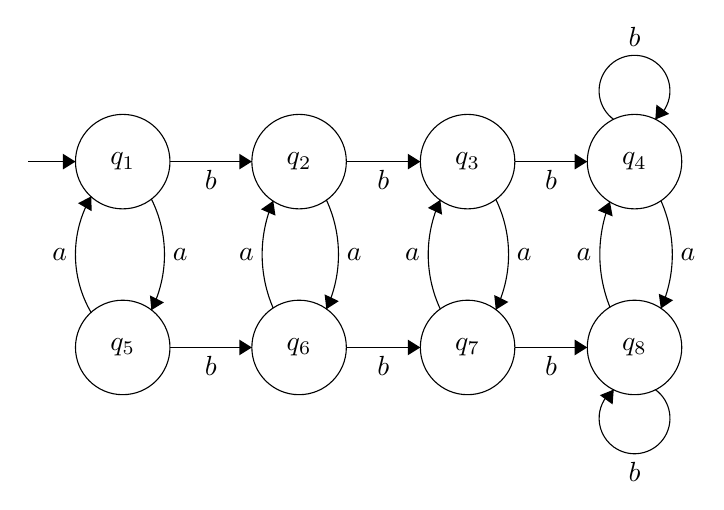
\begin{tikzpicture}[scale=0.2]
                \tikzstyle{every node}+=[inner sep=0pt]
                \draw [black] (18.2,-30.2) circle (3);
                \draw (18.2,-30.2) node {$q_1$};
                \draw [black] (29.4,-30.2) circle (3);
                \draw (29.4,-30.2) node {$q_2$};
                \draw [black] (40.1,-30.2) circle (3);
                \draw (40.1,-30.2) node {$q_3$};
                \draw [black] (50.7,-30.2) circle (3);
                \draw (50.7,-30.2) node {$q_4$};
                \draw [black] (18.2,-42) circle (3);
                \draw (18.2,-42) node {$q_5$};
                \draw [black] (29.4,-42) circle (3);
                \draw (29.4,-42) node {$q_6$};
                \draw [black] (40.1,-42) circle (3);
                \draw (40.1,-42) node {$q_7$};
                \draw [black] (50.7,-42) circle (3);
                \draw (50.7,-42) node {$q_8$};
                \draw [black] (12.2,-30.2) -- (15.2,-30.2);
                \fill [black] (15.2,-30.2) -- (14.4,-29.7) -- (14.4,-30.7);
                \draw [black] (21.2,-30.2) -- (26.4,-30.2);
                \fill [black] (26.4,-30.2) -- (25.6,-29.7) -- (25.6,-30.7);
                \draw (23.8,-30.7) node [below] {$b$};
                \draw [black] (32.4,-30.2) -- (37.1,-30.2);
                \fill [black] (37.1,-30.2) -- (36.3,-29.7) -- (36.3,-30.7);
                \draw (34.75,-30.7) node [below] {$b$};
                \draw [black] (43.1,-30.2) -- (47.7,-30.2);
                \fill [black] (47.7,-30.2) -- (46.9,-29.7) -- (46.9,-30.7);
                \draw (45.4,-30.7) node [below] {$b$};
                \draw [black] (21.2,-42) -- (26.4,-42);
                \fill [black] (26.4,-42) -- (25.6,-41.5) -- (25.6,-42.5);
                \draw (23.8,-42.5) node [below] {$b$};
                \draw [black] (32.4,-42) -- (37.1,-42);
                \fill [black] (37.1,-42) -- (36.3,-41.5) -- (36.3,-42.5);
                \draw (34.75,-42.5) node [below] {$b$};
                \draw [black] (43.1,-42) -- (47.7,-42);
                \fill [black] (47.7,-42) -- (46.9,-41.5) -- (46.9,-42.5);
                \draw (45.4,-42.5) node [below] {$b$};
                \draw [black] (20.016,-32.566) arc (26.61336:-26.61336:7.89);
                \fill [black] (20.02,-39.63) -- (20.82,-39.14) -- (19.93,-38.7);
                \draw (21.35,-36.1) node [right] {$a$};
                \draw [black] (16.2,-39.792) arc (-149.60685:-210.39315:7.298);
                \fill [black] (16.2,-32.41) -- (15.36,-32.84) -- (16.23,-33.35);
                \draw (14.7,-36.1) node [left] {$a$};
                \draw [black] (27.758,-39.508) arc (-156.62367:-203.37633:8.589);
                \fill [black] (27.76,-32.69) -- (26.98,-33.23) -- (27.9,-33.63);
                \draw (26.55,-36.1) node [left] {$a$};
                \draw [black] (31.131,-32.63) arc (25.00279:-25.00279:8.211);
                \fill [black] (31.13,-39.57) -- (31.92,-39.06) -- (31.02,-38.63);
                \draw (32.4,-36.1) node [right] {$a$};
                \draw [black] (38.369,-39.57) arc (-154.99721:-205.00279:8.211);
                \fill [black] (38.37,-32.63) -- (37.58,-33.14) -- (38.48,-33.57);
                \draw (37.1,-36.1) node [left] {$a$};
                \draw [black] (41.888,-32.587) arc (26.08939:-26.08939:7.989);
                \fill [black] (41.89,-39.61) -- (42.69,-39.11) -- (41.79,-38.67);
                \draw (43.2,-36.1) node [right] {$a$};
                \draw [black] (49.143,-39.452) arc (-158.12288:-201.87712:8.996);
                \fill [black] (49.14,-32.75) -- (48.38,-33.3) -- (49.31,-33.68);
                \draw (47.99,-36.1) node [left] {$a$};
                \draw [black] (52.373,-32.671) arc (23.9343:-23.9343:8.452);
                \fill [black] (52.37,-39.53) -- (53.15,-39) -- (52.24,-38.59);
                \draw (53.6,-36.1) node [right] {$a$};
                \draw [black] (49.377,-27.52) arc (234:-54:2.25);
                \draw (50.7,-22.95) node [above] {$b$};
                \fill [black] (52.02,-27.52) -- (52.9,-27.17) -- (52.09,-26.58);
                \draw [black] (52.023,-44.68) arc (54:-234:2.25);
                \draw (50.7,-49.25) node [below] {$b$};
                \fill [black] (49.38,-44.68) -- (48.5,-45.03) -- (49.31,-45.62);
            \end{tikzpicture}

    \end{itemize}

\end{homeworkProblem}
\clearpage

%----------------------------------------------------------------------------------------

\end{document}
